\everymath{\displaystyle}
\documentclass{beamer}
% \documentclass[handout]{beamer}

%\usepackage[pdftex]{color,graphicx}
\usepackage{amsmath,amssymb,amsfonts}

\mode<presentation>
{
  % \usetheme{Darmstadt}
  % \usetheme[hideothersubsections]{Hannover}
  % \usetheme[hideothersubsections]{Goettingen}
  \usetheme[hideothersubsections, right]{Berkeley}

  \usecolortheme{seahorse}
  % \usecolortheme{dolphin}
  \usecolortheme{rose}
  % \usecolortheme{orchid}

  \useinnertheme[shadow]{rounded}

  \setbeamercovered{transparent}
  % or whatever (possibly just delete it)
}

\mode<handout>{
  \setbeamercolor{background canvas}{bg=black!5}
  \usepackage{pgfpages}
  \pgfpagesuselayout{4 on 1}[a4paper,border shrink=5mm, landscape]
}

\usepackage[brazilian]{babel}
% or whatever

% \usepackage[latin1]{inputenc}
\usepackage[utf8]{inputenc}
% or whatever

\usepackage{times}
%\usepackage[T1]{fontenc}
% Or whatever. Note that the encoding and the font should match. If T1
% does not look nice, try deleting the line with the fontenc.


\title%[] % (optional, use only with long paper titles)
{Inferência II}

\subtitle
{Inferências com amostras pequenas} % (optional)

\author%[] % (optional, use only with lots of authors)
{Felipe Figueiredo}% \and S.~Another\inst{2}}
% - Use the \inst{?} command only if the authors have different
%   affiliation.

\institute[INTO] % (optional, but mostly needed)
{Instituto Nacional de Traumatologia e Ortopedia
}
  % \inst{1}%
  % Department of Computer Science\\
  % University of Somewhere
  % \and
  % \inst{2}%
  % Department of Theoretical Philosophy\\
  % University of Elsewhere}
% - Use the \inst command only if there are several affiliations.
% - Keep it simple, no one is interested in your street address.

\date%[] % (optional)
{}

% \subject{Talks}
% This is only inserted into the PDF information catalog. Can be left
% out. 



% If you have a file called "university-logo-filename.xxx", where xxx
% is a graphic format that can be processed by latex or pdflatex,
% resp., then you can add a logo as follows:

\pgfdeclareimage[height=1.6cm]{university-logo}{../logo}
\logo{\pgfuseimage{university-logo}}



% Delete this, if you do not want the table of contents to pop up at
% the beginning of each subsection:
\AtBeginSubsection[]
%\AtBeginSection[]
{
  \begin{frame}<beamer>{Sumário}
    \tableofcontents[currentsection,currentsubsection]
  \end{frame}
}


% If you wish to uncover everything in a step-wise fashion, uncomment
% the following command: 

\beamerdefaultoverlayspecification{<+->}


\begin{document}

\begin{frame}
  \titlepage
\end{frame}

\begin{frame}{Sumário}
  \tableofcontents
  % You might wish to add the option [pausesections]
\end{frame}


%% Template
% \section{}

% \subsection{}

% \begin{frame}{}
%   \begin{itemize}
%   \item 
%   \end{itemize}
% \end{frame}

% \begin{frame}
%   \begin{columns}
%     \begin{column}{5cm}
%     \end{column}
%     \begin{column}{5cm}
%     \end{column}
%   \end{columns}
% \end{frame}

% \begin{frame}{}
%   \includegraphics[height=0.4\textheight]{file1}
%   \includegraphics[height=0.4\textheight]{file2}
%   \includegraphics[height=0.4\textheight]{file3}
%   \begin{figure}
%     \caption{}
%   \end{figure}
% \end{frame}

% \begin{frame}{}
%   \begin{definition}
%   \end{definition}
%   \begin{example}
%   \end{example}
%   \begin{block}{Exercício}
%   \end{block}
% \end{frame}

\section{Recapitulando}

\begin{frame}{Recapitulando}
  \begin{itemize}
  \item Quando vamos fazer uma inferência sobre $\mu$ e
    \alert{sabemos} $\sigma^2$, podemos usar $\sigma$ diretamente no
    intervalo de confiança.
  \item Para isto, consultamos na tabela normal padrão (tabela Z) para
    obter o valor crítico $z_c$
  \item Esse valor crítico representa a probabilidade de que o
    intervalo criado em torno de $\hat{\mu} = \bar{x}$ contenha o
    valor desejado $\mu$.
  \item Na prática, isso raramente acontece (se não sabemos $\mu$,
    raramente saberemos $\sigma^2$).
  \end{itemize}
\end{frame}

\begin{frame}{Recapitulando}
  \begin{itemize}
  \item Uma situação mais realista é quando queremos estimar $\mu$ e
    não sabemos $\sigma$.
  \item Quando temos uma \alert{amostra grande} ($n \ge 30$), podemos
    aproximar $\sigma$ por $s$, e usar $s$ diretamente no cálculo
    da margem de erro
  \item Isso é justificado pelo Teorema Central do Limite (TCL) (e.g.
    vídeo do experimento de Galton).
  \item Consultamos o $z_c$ na tabela Z, usando $s$ como estimador de
    $\sigma$
  \end{itemize}
\end{frame}

\begin{frame}{A tabela Z}
  \begin{itemize}
  \item Para a construção de intervalos de confiança, usamos o nível
    de confiança $c$ (tipicamente $c=0.95$).
  \item Isto é equivalente à \alert{significância} $\alpha = 1-0.95 =
    0.05$
  \item Isto é, a confiança ($c=$ probabilidade de que o IC contenha a
    média) é o complementar da significância ($\alpha=$ probabilidade de que o
    IC não contenha a média).
  \item Pela forma como a tabela é organizada, é mais conveniente
    procurar pela significância $\alpha$ na tabela.
  \item A significância deve ser dividida entre as duas caudas.
  \end{itemize}
\end{frame}

\begin{frame}{A tabela Z}
  \begin{itemize}
  \item A tabela da Normal Padrão mostra os valores sob a curva até o
    ponto $z$ observado (à esquerda de $z$).
  % \item Estes valores correspondem à área à probabilidade de se
  %   encontrar um $Z$ (variável aleatória) com valor menor que $z$
  %   (valor observado): $P(Z<z)$
  \item Cada linha corresponde ao primeiro dígito da área, e cada
    coluna identifica o segundo dígito da área (figura a seguir)
    \begin{example}
      A probabilidade de uma variável aleatória $Z$ ser menor que
      z=0.35 é:
      \begin{displaymath}
        P(Z < 0.35)= 0.6368 = 63.68\%
      \end{displaymath}
    \end{example}
  \end{itemize}
\end{frame}

\begin{frame}{A tabela Z}
  \begin{columns}
    \begin{column}{7cm}
    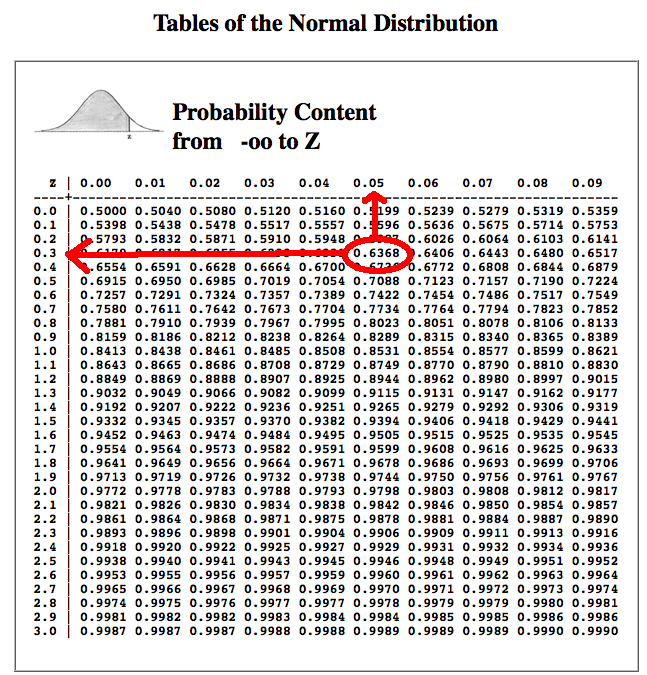
\includegraphics[height=0.9\textheight]{z_table}
    \end{column}
    \begin{column}{5cm}
      \begin{itemize}
      \item $c=95\% = 0.95$
      \item $\alpha = 5\% = 0.05$

      \item $\frac{\alpha}{2} = 2.5\% = 0.0250$

      \item $1-0.025 = 0.9750$%   linha 1.9 e
      % coluna 0.06

      \item Assim, o $z_c$ é 1.96

      \end{itemize}
    \end{column}
  \end{columns}
\end{frame}

\begin{frame}{E se a amostra não for grande?}
  \begin{itemize}
  \item Quando a amostra é pequena, não podemos simplesmente
    substituir $\sigma$ por $s$ na fórmula, pois o erro dessa
    aproximação não é desprezível.
  \item Nesse caso, a média amostral não tem distribuição normal.
  \item Assim precisamos usar uma outra distribuição (tabelada) com a
    distribuição \alert{t de Student}.
  \end{itemize}
\end{frame}


\section{Intervalos de confiança para a média}

\subsection{A distribuição t de Student}

\begin{frame}{A distribuição t de Student}
  \begin{itemize}
  \item Student (pseudônimo de W. S. Gossett [1876-1937], trabalhando
    para a cervejaria Guiness) criou uma distribuição que melhor se
    aproxima dos dados de amostras pequenas
%  \item É semelhante à Normal padrão, mas tem variância maior
  \item Tem um parâmetro \alert{graus de liberdade} (gl) vinculado ao
    tamanho da amostra $n$.
    % \begin{displaymath}
    %   gl = n-1
    % \end{displaymath}
  \end{itemize}
\end{frame}

\begin{frame}{A distribuição t de Student}
  \begin{figure}
    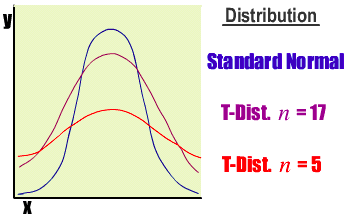
\includegraphics[height=0.7\textheight]{t_graph}
    \caption{A distribuição t de Student}
  \end{figure}
\end{frame}

\begin{frame}{Propriedades da distribuição t}
  \begin{itemize}
  \item A distribuição tem forma de sino (simétrica) assim como a
    Normal padrão Z
  \item Reflete a maior variabilidade inerente às amostras pequenas
  \item O formato da curva depende do tamanho da amostra $n$
  \item Quanto mais graus de liberdade (dados), mais a distribuição
    $t$ se parece com a distribuição $Z$.
  \end{itemize}
\end{frame}

\subsection{Intervalos de confiança para amostras pequenas}

\begin{frame}{Intervalos de confiança para a média}
  \begin{definition}
    A margem de erro usando a estatística $t$ é
    \begin{displaymath}
      E = t_c \times \frac{s}{\sqrt{n}}
    \end{displaymath}
  \end{definition}
  \begin{itemize}
  \item Consultamos a tabela $t$ de Student para encontrar o valor
    crítico $t_c$
  \item Graus de liberdade: \alert{$gl = n-1$} (onde $n$ é o tamanho da
    amostra)
  \end{itemize}
\end{frame}

\begin{frame}{A tabela t}
  \begin{center}
    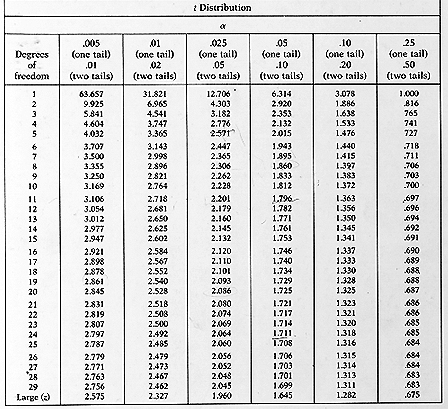
\includegraphics[height=0.9\textheight]{t_table}
  \end{center}
\end{frame}

\begin{frame}{Exemplo}
  \begin{example}
    Considere uma amostra de 10 bebês selecionada de uma população de
    bebês que recebe antiácidos que contém alumínio e são
    frequentemente usados para tratar distúrbios digestivos. A
    distribuição de níveis de alumínio no plasma é conhecida como
    aproximadamente normal, no entanto sua média e desvio padrão não
    são conhecidos. O nível médio de alumínio para a amostra de dez
    bebês é 37.2 $\mu$g/l e desvio-padrão 7.13 $\mu$g/l. Calcule um
    intervalo com 95\% de confiança para a média populacional.
  \end{example}
  (Fonte: Hacker \& Simões, 2008, Fiocruz)
\end{frame}

\begin{frame}{Exemplo}
  \begin{itemize}
  \item $\bar{x}=37.2$
  \item $s=7.13$
  \item $n=10 \Rightarrow gl=9$
  \end{itemize}
  \begin{block}{Solução}
    \begin{displaymath}
      t_c = 2.262
    \end{displaymath}
    \begin{displaymath}
      E = t_c \times \frac{s}{\sqrt{n}}
    \end{displaymath}
    \begin{displaymath}
      E = 2.262 \times \frac{7.13}{\sqrt{10}} \approx 5.1
    \end{displaymath}
    \begin{displaymath}
      IC(95\%) = (37.2 - 5.1 , 37.2 + 5.1 ) = \alert{(32.1 , 42.3)}
    \end{displaymath}
  \end{block}
\end{frame}

\begin{frame}{Exercício}
  \begin{block}{Exercício}
    Num estudo para descrever o perfil dos pacientes adultos atendidos
    no ambulatório de um posto de saúde, uma amostra de \alert{16}
    pacientes adultos foi selecionada ao acaso entre o total de
    pacientes atendidos no posto durante os últimos três anos,
    coletando-se dos prontuários desses pacientes dados relativos à
    idade, à
    escolaridade e a outros fatores de interesse.\\

    Para a variável idade, observou-se uma média amostral de 36.86
    anos com um desvio padrão amostral de 17.79 anos.    
  \end{block}
\end{frame}

\begin{frame}{Exercício}
  \begin{block}{Exercício}
    \begin{enumerate}
    \item Defina a população e a amostra.
    \item Forneça uma estimativa pontual, um intervalo de 90\% de
      confiança e um intervalo de 95\% de confiança para a idade média
      dos adultos atendidos neste ambulatório nos últimos três
      anos. Interprete e compare os intervalos de confiança.
    \end{enumerate}
  \end{block}

  \begin{block}{}
    \begin{columns}
      \begin{column}{5cm}
    \begin{displaymath}
      E = \frac{t_c s}{\sqrt{n}}
    \end{displaymath}
    \begin{displaymath}
      t_c (90\%) = 1.753
    \end{displaymath}
    \begin{displaymath}
      t_c (95\%) = 2.132
    \end{displaymath}
  \end{column}
  \begin{column}{5cm}
    \begin{displaymath}
      \bar{x} = 36.86
    \end{displaymath}
    \begin{displaymath}
      s = 17.79
    \end{displaymath}
    \begin{displaymath}
      n = 16 \Rightarrow gl = 15
    \end{displaymath}
  \end{column}
\end{columns}
\end{block}
\end{frame}

\begin{frame}{Exercício}
  \begin{block}{Solução}
    \begin{itemize}
    \item IC de 90\% (c=0.90)
    \begin{displaymath}
      E = \frac{t_c s}{\sqrt{n}} = \frac{1.753 \times 17.79}{\sqrt{16}}
      \approx 7.80
    \end{displaymath}
    \begin{displaymath}
      IC_{0.90} = \bar{x} \pm E = 36.86 \pm 7.80 = (29.06 , 46.66)
    \end{displaymath}
  \item IC de 95\% (c=0.95)
    \begin{displaymath}
      E = \frac{t_c s}{\sqrt{n}} = \frac{2.132 \times 17.79}{\sqrt{16}}
      \approx 9.48
    \end{displaymath}
    \begin{displaymath}
      IC_{0.95} = \bar{x} \pm E = 36.86 \pm 9.48 = (27.38 , 46.34)
    \end{displaymath}
  \end{itemize}
\end{block}
\end{frame}


\section{Resumo}

\begin{frame}{Resumo}
  Para construir um intervalo de confiança para a média $\mu$ devemos
  considerar as informações e dados disponíveis:
  \begin{itemize}
  \item Se soubermos $\sigma$, usamos a tabela Z
    ($z_c$)
    \begin{displaymath}
      E = z_c \frac{\sigma}{\sqrt{n}}
    \end{displaymath}
  \item Se não soubermos $\sigma$, mas se $n$ é grande ($n \ge 30$),
    usamos a tabela Z ($z_c$)
    \begin{displaymath}
      E = z_c \frac{s}{\sqrt{n}}
    \end{displaymath}
  \item Se não soubermos $\sigma$, mas e se $n$ é pequeno ($n < 30$),
    usamos a tabela t ($t_c$)
    \begin{displaymath}
      E = t_c \frac{s}{\sqrt{n}}
    \end{displaymath}
  \end{itemize}
\end{frame}


\end{document}
